\documentclass{article} % For LaTeX2e
\usepackage{nips14submit_e,times}
\usepackage{amsmath}
\usepackage{amsthm}
\usepackage{amssymb}
\usepackage{mathtools}
\usepackage{hyperref}
\usepackage{url}
\usepackage{algorithm}
\usepackage[noend]{algpseudocode}
%\documentstyle[nips14submit_09,times,art10]{article} % For LaTeX 2.09

\usepackage{graphicx}
\usepackage{caption}
\usepackage{subcaption}

\def\eQb#1\eQe{\begin{eqnarray*}#1\end{eqnarray*}}
\def\eQnb#1\eQne{\begin{eqnarray}#1\end{eqnarray}}
\providecommand{\e}[1]{\ensuremath{\times 10^{#1}}}
\providecommand{\pb}[0]{\pagebreak}
\DeclarePairedDelimiter\ceil{\lceil}{\rceil}
\DeclarePairedDelimiter\floor{\lfloor}{\rfloor}

\newcommand{\E}{\mathrm{E}}
\newcommand{\Var}{\mathrm{Var}}
\newcommand{\Cov}{\mathrm{Cov}}

\def\Qb#1\Qe{\begin{question}#1\end{question}}
\def\Sb#1\Se{\begin{solution}#1\end{solution}}

\newenvironment{claim}[1]{\par\noindent\underline{Claim:}\space#1}{}
\newtheoremstyle{quest}{\topsep}{\topsep}{}{}{\bfseries}{}{ }{\thmname{#1}\thmnote{ #3}.}
\theoremstyle{quest}
\newtheorem*{definition}{Definition}
\newtheorem*{theorem}{Theorem}
\newtheorem*{lemma}{Lemma}
\newtheorem*{question}{Question}
\newtheorem*{preposition}{Preposition}
\newtheorem*{exercise}{Exercise}
\newtheorem*{challengeproblem}{Challenge Problem}
\newtheorem*{solution}{Solution}
\newtheorem*{remark}{Remark}
\usepackage{verbatimbox}
\usepackage{listings}
\title{Probabilistic Method: \\
Problem Set I}


\author{
Youngduck Choi \\
CIMS \\
New York University\\
\texttt{yc1104@nyu.edu} \\
}


% The \author macro works with any number of authors. There are two commands
% used to separate the names and addresses of multiple authors: \And and \AND.
%
% Using \And between authors leaves it to \LaTeX{} to determine where to break
% the lines. Using \AND forces a linebreak at that point. So, if \LaTeX{}
% puts 3 of 4 authors names on the first line, and the last on the second
% line, try using \AND instead of \And before the third author name.

\newcommand{\fix}{\marginpar{FIX}}
\newcommand{\new}{\marginpar{NEW}}

\nipsfinalcopy % Uncomment for camera-ready version

\begin{document}


\maketitle

\begin{abstract}
This work contains solutions to the problem set I
of Probabilistic Method 2016 at Courant Institute of Mathematical Sciences.
\end{abstract}

\bigskip

\begin{question}[1]
\hfill
\begin{figure}[h!]
  \centering
    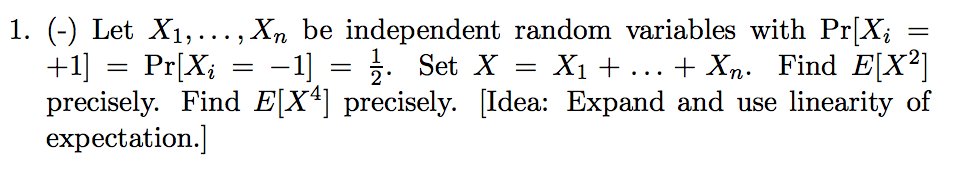
\includegraphics[width=1\textwidth]{PM-2-1.png}
\end{figure}
\end{question}
\begin{solution}
By expanding the terms, using linearity of expectation,  we have
\eQb
E[X^2] &=& E[(\sum_{i=1}^{n} X_i)^2] \\
&=& E[\sum_{i=1}^{n} X_i^2] + 2\sum_{1\leq i<j \leq n}X_i X_j] \\
&=& \sum_{i=1}^{n} E[X_i^2] + 2\sum_{1 \leq i < j \leq n} E[X_i X_j]. \\
\eQe
Observe that 
\eQb
E[X_i^2] &=& 1^2 \dfrac{1}{2} + (-1)^2 \dfrac{1}{2} \\
&=& \dfrac{1}{2} + \dfrac{1}{2} = 1.
\eQe
From the independence assumption, we have
\eQb
E[X_i X_j ] &=& E[X_i] E[X_j] = 0,
\eQe
for $i \neq j$. 
Therefore, by substitution to the previous equality, we have
\eQb
E[X^2] &=& n.
\eQe
Now, for the $E[X^4]$, we note that the terms with $E[X_i]$ terms will all be $0$.
Therefore, we directly obtain
\eQb
E[X^4] &=& \sum_{i=1}^{n} E[X_i]^4 + {4 \choose 2}E[\sum_{1\leq i \leq j \leq n}
X_i^2 X_j^2] \\
&=& n + {4 \choose 2}{n \choose 2} = 3n^2 - 2n. 
\eQe
\hfill $\qed$


\end{solution}

\bigskip

\begin{question}[2]
\hfill
\begin{figure}[h!]
  \centering
    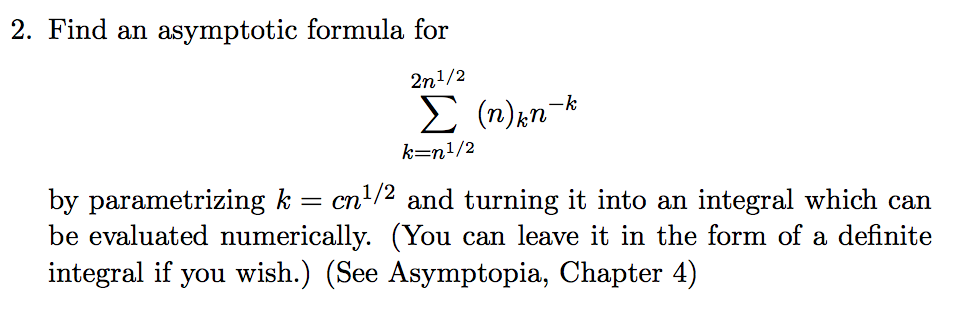
\includegraphics[width=1\textwidth]{PM-2-2.png}
\end{figure}
\end{question}
\begin{solution}
By definition, we have
\eQb
(n)_{k}k^{-k} &=& \dfrac{n!}{(n-k)!}n^{-k} \\
&=& {n \choose k} k! n^{-k}.
\eQe
As we are given $k \sim c\sqrt{n}$, from Asymtopia, we have
\eQb
{n \choose k} \sim e^{-\frac{c^2}{2}} \dfrac{n^k}{k!}.
\eQe
By the Stirling's formula, it immediately follows that
\eQb
(n)_{k} n^{-k} &\sim& e^{-\frac{c^2}{2}} \dfrac{n^k}{k!} k! n^{-k} = e^{-\frac{c^2}{2}}.
\eQe
Using the integration given in Asymtopia, we have
\eQb
\sum_{k=\sqrt{n}}^{2\sqrt{n}} (n)_{k}n^{-k} &\sim& \int_{1}^{2} \sqrt{n} e^{-\frac{c^2}{2}} dc \\
&\sim& 0.34\sqrt{n},
\eQe
as required. \hfill $\qed$

\end{solution}

\newpage

\begin{question}[3]
\hfill
\begin{figure}[h!]
  \centering
    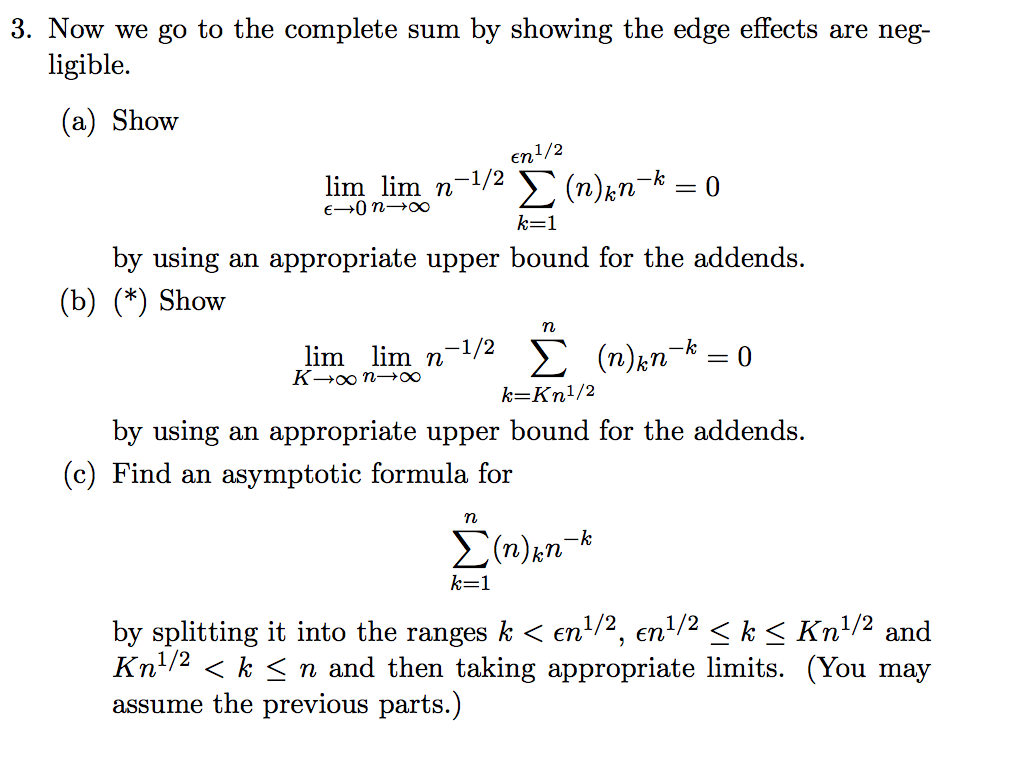
\includegraphics[width=1\textwidth]{PM-2-3.png}
\end{figure}
\end{question}
\begin{solution}
\textbf{(a)} By definition of $(n)_k$, it follows that
\eQb
\dfrac{1}{\sqrt{n}} \sum_{k=1}^{\epsilon \sqrt{n}} (n)_{k} n^{-k} &\leq& \dfrac{1}{\sqrt{n}}
\dfrac{1}{\sqrt{n}} \sum_{k=1}^{\epsilon \sqrt{n}} 1 = \epsilon, 
\eQe
which goes to $0$ as $\epsilon \to 0$.  

\end{solution}

\newpage

\begin{question}[4]
\hfill
\begin{figure}[h!]
  \centering
    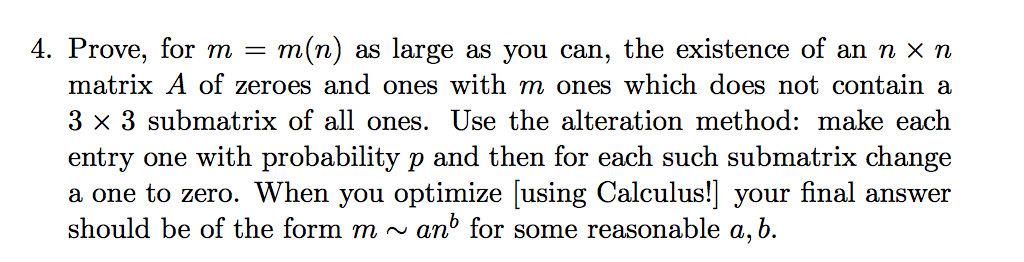
\includegraphics[width=1\textwidth]{PM-2-4.png}
\end{figure}
\end{question}
\begin{solution}
Consider a random $n \times n$ matrix, $M_{n}$, obtained 
by assigning each entry independently either $1$ or $0$, where the probability 
of assigning $1$ is $p$. Let $X$ be a random variable, which counts
number of $1$s in the matrix, and $Y$ be a random variable, which counts 
number of $3 \times 3$ submatrices of all $1$s. 
For any $3 \times 3$ submatrix $S$, let $Y_S$ be the
indicator random variable for the event for which the submatrix $S$ has entries of all $1$s,
so that $Y = \sum Y_{S}$. By Linearity of Expectation, we have
\eQb
E[Y] &=& \sum E[Y_S] = {n \choose 3}^2 p^{9}. \\
\eQe 
Clearly, $E[X] = n^2 p$. Therefore, again by Linearity of Expectation, it follows that
\eQb
E[X - Y] &=& n^2 p - {n \choose 3}^2 p^{9} = f(p). 
\eQe
Hence, there exists a random assignment, for which the number of $1$s minus 
the number of $3 \times 3$ submatrices of $1$ is at least $f(p)$.
Fix such a coloring. Select one entry from each submatrix and change to $0$. This leaves
the matrix with at least $f(p)$ entries with $1$. 

\smallskip

We now optimize this result by maximizing $f(p)$ with respect to $p$. Observe that $f$ 
is concave with respect to $p \in [0,1]$. Solving for the local maxima by setting the
first-order derivative equals to $0$, we get that $f$ is maximized at 
$p^* = (\dfrac{n^2}{9{n \choose 3}^2})^{\frac{1}{8}} = (\dfrac{2}{(n-1)(n-2)})^{\frac{1}{4}}$.
Substituting $p^*$ back into $f(p)$, we obtain
\eQb
f(p^*) &=& n^2(\dfrac{2}{(n-1)(n-2)})^{\frac{1}{4}} - {n \choose 3}^2 
\dfrac{n^2}{9 {n \choose 3}^2}(\dfrac{2}{(n-1)(n-2)})^{\frac{1}{4}} \\
&=& \dfrac{8}{9}n^2(\dfrac{2}{(n-1)(n-2)})^{\frac{1}{4}} \\ 
&\sim& \dfrac{8}{9}2^{\frac{1}{4}}n^{\frac{3}{2}}. 
\eQe
Recall that $m(n)$ be the minimum number of $1$ in $n \times n$ matrix, such that
there must exist a $3 \times 3$ submatrix of all $1$s.
We have shown that $m(n) = \Omega(n^{\frac{3}{2}})$.
\hfill $\qed$
\end{solution}

\newpage

\begin{question}[5]
\hfill
\begin{figure}[h!]
  \centering
    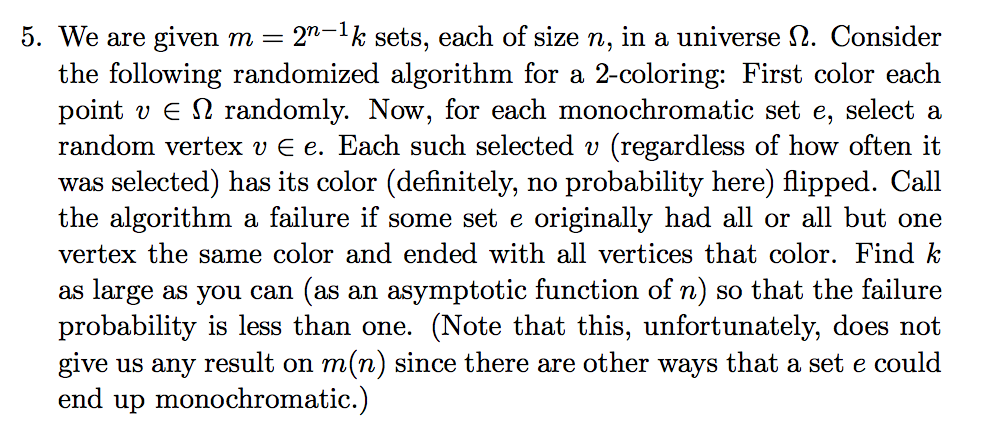
\includegraphics[width=1\textwidth]{PM-2-5.png}
\end{figure}
\end{question}
\begin{solution}
Note that we use the langauge of $n-$uniform hypergraph, which is an equivalent problem 
to the problem under consideration.
Before proceeding with the main part of the proof, we define an object, called
a conflicting pair, and peacebreaker, in a two-coloring scheme. 

\smallskip

\begin{definition}[5.1]
An ordered pair of edges $(e,f)$ is said to be a \textbf{conflicting pair}
, if $e$ is monochromatic with some color $k$, and for some $v \in e \cap f$,
$f \setminus \{ v \}$ is monochromatic
with the color  not $k$. We call the vertex $v$ the \textbf{peacebreaker} of $(e,f)$. 
\end{definition}

\smallskip

We now consider the randomized algorithm. Fix $(e,f)$ an ordered pair of edges from 
the hypergraph.
Consider an event, where after the initial coloring, $(e,f)$ is a conflicting pair with 
a peacebreaker $v$, and at the second stage chooses the peacebreaker $v$ 
to flip its color, exactly when it reviews $e$. We denote such event 
as $T_{(e,f)}$. We first note that if $e$ and $f$ have a number of
common vertices not equal to $1$, we have that $P(T_{(e,f)}) = 0$, as
no matter what coloring is given to $e$ and $f$, they cannot be a conflicting pair. 
Now, for the case where $e,f$ exactly have one vertex in common,
the probability of $T_{(e,f)}$ is given by
\eQb
P(T_{(e,f)}) &=&  
P(\{ (e,f) \text{ is a conflicting pair after the i.c.} \}) \\ 
&\cdot& P(\{ v \text{ is chosen at the review of $e$ } \} | 
\{ (e,f) \text{ is a conflicting pair after the i.c.} \})  \\
&=& 2^{2-2n} n^{-1},
\eQe
where i.c. denotes the initial coloring, prior to the second round of flipping colors.
Therefore, $P(T_{(e,f)})$ in general can be upper-bounded as follows:
\eQb
P(T_{(e,f)}) &\leq& 2^{2-2n}n^{-1},
\eQe
with equality being achieved when $e$ and $f$ share exactly one vertex.

\bigskip

\begin{lemma}[5.2. Failure implies 
$\mathbf{\bigcup_{(e,f) \in E \times E} T_{(e,f)}}$] 
\textit{
The algorithm fails, only if there exists a conflicting pair $(e,f)$
with its peacebreaker $v$ chosen at the second stage at the review of $e$.}
\end{lemma}
\begin{proof}
Observe that any monochromatic edge after the initial coloring cannot cause a failure, 
because at least one of its vertex will be chosen to flip the color at the second stage. 
Hence, failure occurs, if only if there exists an edge, having all but one color
monochromatic, end up having a monochromatic coloring with the majority color.
Now, for any edge, having all but one color monochromatic, will end up having the 
monochromatic coloring, only if there exists a monochromatic edge containing the one vertex
with the opposite color and the vertex is chosen to be fliped at the second stage of 
the algorithm, as the algorithm reviews the monochromatic edge.
This is precisely the identification of a conflicting pair with its 
peacebreaker. Hence, we have proven the claim.
\end{proof}

\newpage

By the established lemma, we obtain
\eQb
\{ \text{ failure} \} &\implies & \bigcup_{(e,f) \in E \times E} T_{(e,f)}. 
\eQe
As there are $m^2$ ordered pairs of edges in the hypergraph, by the above equality,
and the subadditivity of probability, we obtain
\eQb
P(\{ \text{ failure }\})  
&\leq& P(\bigcup_{(e,f) \in E\times E} T_{(e,f)}) \\ 
&\leq& \sum_{(e,f) \in E \times E} P(T_{(e,f)} ) \\ 
&\leq& m^2 2^{2 - 2n} n^{-1}, \\
\eQe
where $E$ denotes the edge set. If $m^2 2^{2 -2n}n^{-1} < 1$, we can ensure that
the failure probability is less than $1$. Substituting $2^{n-1}k$ for $m$, we have
\eQb
(2^{n-1}k)^2 2^{2-2n} n^{-1} < 1,
\eQe
which is equivalent to $ k < \sqrt{n}$. Hence, by taking $k = \floor{\sqrt{n}} - 1$, we can
have a failure probability less than $1$. We have shown that $k = \Omega(\sqrt{ n})$.
One should note that this bound is higher by a factor of $\ln(n)$ compared to 
the state of the art lower bound, established Kozik et al. As the note mentions,
this is not a surprise, since the "failure" defined through this procedure is not
inclusive enough to capture all possible ways an edge $e$ could end up monochromatic.
\hfill $\qed$


\end{solution}

\newpage

\begin{question}[6]
\hfill
\begin{figure}[h!]
  \centering
    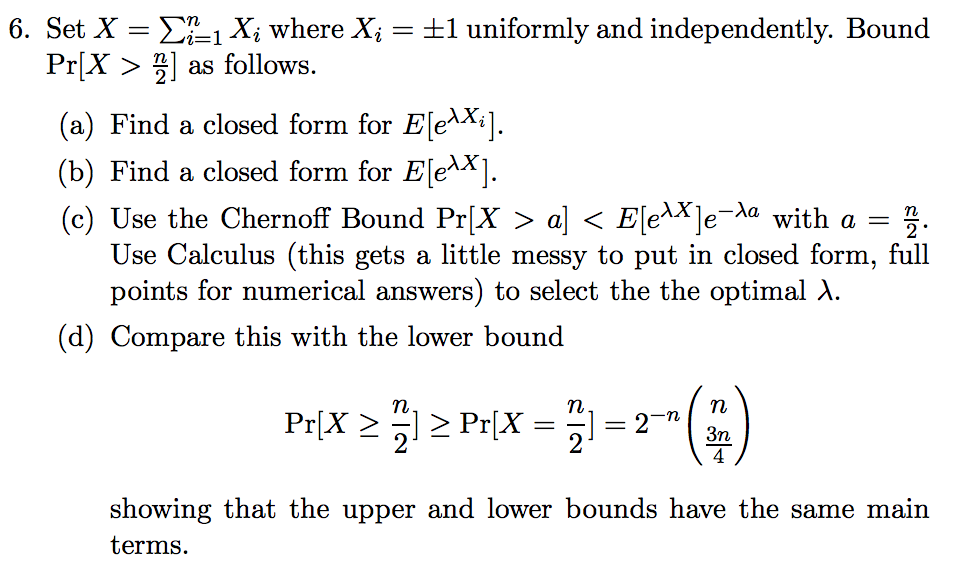
\includegraphics[width=1\textwidth]{PM-2-6.png}
\end{figure}
\end{question}
\begin{solution}
\textbf{(a)}
By definition of expectation, it follows that
\eQb
E[e^{\lambda x_i}] &=& \dfrac{e^{\lambda} + e^{-\lambda}}{2} = \cosh(\lambda). \\
\eQe

\bigskip
 
\textbf{(b)}
By using the fact that expectation of product of independent random variables is a 
product of expectations and $(b)$, we have
\eQb
E[e^{\lambda X}] &=& \prod_{i=1}^{n}E[e^{\lambda X_i}] \\
&=& (\cosh(\lambda))^n.
\eQe

\bigskip

\textbf{(c)} 
By the use of Chernoff bound, we obtain
\eQb
P(X > \dfrac{n}{2}) < (\dfrac{e^{\frac{\lambda}{2}} + e^{-\frac{3\lambda}{2}}}{2})^n.
\eQe
Let $f(\lambda) = e^{\frac{\lambda}{2}} + e^{-\frac{3\lambda}{2}}$. By taking the
first order derivative and setting it equal to $0$, we obtain $e^{\frac{\lambda}{2}} 
= 3e^{-\frac{3\lambda}{2}}$. Solving this equality, we get the optimal $\lambda$, 
$\lambda^*$, is
$\dfrac{\ln(3)}{2}$. Plugging it back in, we get that $f(\lambda^*) = 3^{\frac{1}{4} + \frac{3}{4}}$.
Hence, it follows that
\eQb
P(X > \dfrac{n}{2}) < (\dfrac{2}{3^{\frac{3}{4}}})^n ,
\eQe
as required.

\bigskip

\textbf{(d)} Using the Stirling's formula, we have
\eQb
P(X \geq \dfrac{n}{2}) &\leq& P(X = \dfrac{n}{2}) \\
&=& 2^{-n}{n \choose \frac{3n}{4}} \\
&=& 2^{-n}\dfrac{n!}{(\frac{3n}{4})!(\frac{n}{4})!} \\
&\sim& 2^{-n}\dfrac{\sqrt{2\pi n} (\frac{n}{e})^n }{\sqrt{2\pi \frac{3n}{4}} 
(\frac{3n}{4e})^{\frac{3n}{4}} \sqrt{2\pi \frac{n}{4} }(\frac{n}{4e})^{\frac{n}{4}}} \\
&=& \dfrac{2\sqrt{2}}{\sqrt{3\pi n}}(\dfrac{2}{3^{\frac{3}{4}}})^n. 
\eQe
The main terms are the same for the upper bound and the lower bound as remarked.
\hfill $\qed$ 

\end{solution}

\end{document}
